\documentclass[aps, prb, twocolumn, a4paper, floatfix, reprint]{revtex4-2}
\usepackage[%
    margin=10mm,% ако не си принтира 10мм не изглежда грозно, а може да събереш повече текст
    % showframe=true,%
    ]{geometry}
\usepackage[T1,T2A]{fontenc}
\usepackage[utf8]{inputenc}
\usepackage[main=bulgarian, english]{babel}
\usepackage{float}
\AtBeginDocument{\selectlanguage{bulgarian}}
\newcommand{\degree}{^{\circ}}
\usepackage{amsmath}
\usepackage{graphics}
\usepackage{graphicx}
\graphicspath{{.}}
\newcommand{\abs}[1]{\lvert#1\rvert}
\let\phi\varphi
\usepackage{booktabs} % от тук се използва само \midrule може и без него 
%\usepackage{adjustbox} % това може да се използва, за да „смаляваш“ широки таблици
%\usepackage{tabularx} % дефинира колона X в среда tabularx която добавя празно място така че цялата таблица да запълни определена ширина
\usepackage{dcolumn}
\newcolumntype{d}[1]{D{.}{.}{#1}}
\usepackage[unicode=true,pdfusetitle]{hyperref}


\makeatletter
\renewcommand{\Dated@name}{}%
\makeatother



\begin{document}
\title{Еластично огъване}
\author{Васил Николов}
\noaffiliation
\date{21.11.2021}
\maketitle

\section{Цел на упражнението}
Да се изследва зависимостта на деформацията на метална линия като функция на приложена сила в средата на линията, и да се измери модулът на Юнг на стоманата.


\section{Експериментална установка}
Тънка метална линия с дебелина $a=(1.52 \pm 0.02)$ mm и широчина $b=(24.05 \pm 0.05)$ mm е окачена от две страни на два метални ръба, разстоянието между които е $l_0 = (45.9 \pm 0.1)$ cm. Над средата на линията има микрометър с точност $0.002$ mm с проводящ връх, така че когато се докосне до линията да се затвори верига, която индикира, че линията и върхът на микрометъра са допряни. Така може да се измери с голяма точност деформацията на линията. Сила върху линийката се прилага като се закачат различни тежести на средата на линийката.

\section{Теоретична обосновка}
Може да се изведе, че при така описаната установка деформацията зависи по следният начин от приложената сила и параметрите на системата:
\begin{equation} \label{eq:1}
    \Delta h=\frac{l_0^3 G}{4E a^3 b}
\end{equation}
където $G$ е силата на тежестта на закачената маса и $E$ е модулът на Юнг на материала, от който е направена линийката. При много измервания можем да направим графика на зависимостта на 
\begin{gather*} \label{eq:2}
    y=\Delta h; \ \ x = m \\
    \frac{dy}{dx} = \frac{l_0^3 g}{4E a^3 b} \\
    E = \frac{l_0^3 g}{4a^3 b \frac{dy}{dx}} \tag{2}
\end{gather*}

\section{Експериментални данни и резултати}
По гореописания метод се мери деформацията на линийката като функция на окачетата маса. 
В рамките на грешката двете стойности съвпадат, както се и очаква от закона за запазване на импулса.
\begin{table}[H]
    \caption{\label{tab:1} Зависимост на деформацията от окачената маса}
    \begin{ruledtabular}
        \begin{tabular}{rd{1.2}d{2.2}}
            \multicolumn{1}{c}{№}             &
            \multicolumn{1}{c}{$m$, g} &
            \multicolumn{1}{c}{$\Delta h$, mm}                \\[2pt]
            \midrule
            1 & 0    & 0     \\
            2 & 104  & 1.738 \\
            3 & 97   & 1.37  \\
            4 & 100  & 1.382 \\
        \end{tabular}
    \end{ruledtabular}
\end{table}

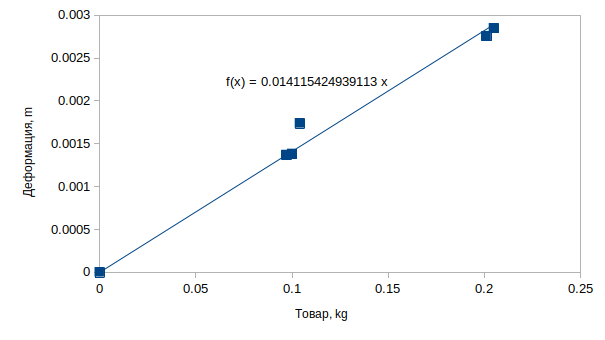
\includegraphics[width=0.9\columnwidth,keepaspectratio=true]{chart_oguvane_2}

На графиката $\frac{dy}{dx}= 1.41*10^{-2} \ m \ kg^{-1} \pm 2\%$. Оценяме грешката на производната по това колко далеч от правата са точките. Заедно с грешките на останалите резултати получаваме
\begin{equation*}
    E = 201 \ GPa \pm 4\%
\end{equation*}
което се вписва добре в табличните стойности от $190 \textnormal{ до } 215 \ GPa$.

\end{document}